\documentclass[12pt,a4paper]{article}

% ============================================
% PACKAGES
% ============================================
\usepackage[utf8]{inputenc}
\usepackage[T1]{fontenc}
\usepackage[french]{babel}
\usepackage{amsmath, amsfonts}
\usepackage{graphicx}
\usepackage{float}
\usepackage{booktabs}
\usepackage{geometry}
\usepackage{xcolor}
\usepackage{listings}
\usepackage{hyperref}
\usepackage{fancyhdr}

% ============================================
% CONFIGURATION
% ============================================
\geometry{left=2.5cm, right=2.5cm, top=2.5cm, bottom=2.5cm}
\hypersetup{colorlinks=true, linkcolor=blue, urlcolor=cyan}

% Configuration des listings pour R
\lstdefinestyle{Rstyle}{
    language=R,
    basicstyle=\ttfamily\footnotesize,
    keywordstyle=\color{blue}\bfseries,
    commentstyle=\color{green!60!black},
    numbers=left,
    numberstyle=\tiny\color{gray},
    backgroundcolor=\color{gray!10},
    frame=single,
    breaklines=true,
    tabsize=2,
    literate={é}{{\'e}}1 {è}{{\`e}}1 {ê}{{\^e}}1 {à}{{\`a}}1 {ù}{{\`u}}1
}

% Configuration des listings pour Python
\lstdefinestyle{Pythonstyle}{
    language=Python,
    basicstyle=\ttfamily\footnotesize,
    keywordstyle=\color{blue}\bfseries,
    commentstyle=\color{green!60!black},
    numbers=left,
    numberstyle=\tiny\color{gray},
    backgroundcolor=\color{yellow!10},
    frame=single,
    breaklines=true,
    tabsize=4,
    literate={é}{{\'e}}1 {è}{{\`e}}1 {ê}{{\^e}}1 {à}{{\`a}}1 {ù}{{\`u}}1
}

% En-tête
\pagestyle{fancy}
\fancyhf{}
\rhead{GMM2 - Exercice 3}
\lhead{Analyse des Correspondances Multiples}
\cfoot{\thepage}

% ============================================
% DOCUMENT
% ============================================
\begin{document}

% ============================================
% TITRE
% ============================================
\begin{center}
    \rule{\linewidth}{0.5mm}\\[0.4cm]
    {\Huge \textbf{EXERCICE 3}}\\[0.3cm]
    {\Large \textbf{Analyse des Correspondances Multiples (ACM)}}\\[0.2cm]
    {\large Base de données : Adult Clean}\\[0.1cm]
    \rule{\linewidth}{0.5mm}\\[1cm]
\end{center}

% ============================================
% PRÉSENTATION DES DONNÉES
% ============================================
\section{Présentation des Données}

\subsection{Description}

La base de données \textbf{Adult Clean} est un extrait simplifié du célèbre dataset "Adult" (Census Income). Elle contient des informations sociodémographiques sur des individus et vise à étudier les relations entre différentes caractéristiques qualitatives.

\begin{itemize}
    \item \textbf{Nombre d'observations} : 8 individus
    \item \textbf{Nombre de variables} : 5 variables qualitatives
    \item \textbf{Nombre total de modalités} : 14 modalités
\end{itemize}

\subsection{Description des variables}

\begin{table}[H]
\centering
\caption{Variables et leurs modalités}
\begin{tabular}{|l|c|l|}
\hline
\textbf{Variable} & \textbf{Nb modalités} & \textbf{Modalités} \\
\hline
Sex & 2 & Male, Female \\
Education & 4 & Bachelors, HS-grad, Masters, PhD \\
Marital\_status & 3 & Married, Single, Divorced \\
Occupation & 3 & Tech, Service, Exec \\
Income & 2 & $\leq$50K, $>$50K \\
\hline
\end{tabular}
\end{table}

\subsection{Tableau des données}

\begin{table}[H]
\centering
\caption{Données brutes}
\footnotesize
\begin{tabular}{|c|l|l|l|l|l|}
\hline
\textbf{Ind.} & \textbf{Sex} & \textbf{Education} & \textbf{Marital\_status} & \textbf{Occupation} & \textbf{Income} \\
\hline
1 & Male & Bachelors & Married & Tech & $\leq$50K \\
2 & Female & HS-grad & Single & Service & $>$50K \\
3 & Female & Masters & Married & Exec & $>$50K \\
4 & Male & HS-grad & Divorced & Service & $\leq$50K \\
5 & Male & PhD & Married & Exec & $>$50K \\
6 & Female & Bachelors & Single & Tech & $\leq$50K \\
7 & Male & Masters & Divorced & Tech & $>$50K \\
8 & Female & HS-grad & Married & Service & $\leq$50K \\
\hline
\end{tabular}
\end{table}

\subsection{Statistiques descriptives}

\subsubsection{Répartition par variable}

\begin{table}[H]
\centering
\caption{Effectifs et pourcentages par modalité}
\begin{tabular}{|l|l|c|c|}
\hline
\textbf{Variable} & \textbf{Modalité} & \textbf{Effectif} & \textbf{Pourcentage} \\
\hline
\multirow{2}{*}{Sex} & Male & 4 & 50\% \\
 & Female & 4 & 50\% \\
\hline
\multirow{4}{*}{Education} & HS-grad & 3 & 37.5\% \\
 & Bachelors & 2 & 25\% \\
 & Masters & 2 & 25\% \\
 & PhD & 1 & 12.5\% \\
\hline
\multirow{3}{*}{Marital\_status} & Married & 4 & 50\% \\
 & Single & 2 & 25\% \\
 & Divorced & 2 & 25\% \\
\hline
\multirow{3}{*}{Occupation} & Tech & 3 & 37.5\% \\
 & Service & 3 & 37.5\% \\
 & Exec & 2 & 25\% \\
\hline
\multirow{2}{*}{Income} & $\leq$50K & 4 & 50\% \\
 & $>$50K & 4 & 50\% \\
\hline
\end{tabular}
\end{table}

\textbf{Observations :}
\begin{itemize}
    \item \textbf{Sex} : Répartition équilibrée (50\% hommes, 50\% femmes)
    \item \textbf{Education} : Prédominance du niveau HS-grad (37.5\%), suivi de Bachelors et Masters
    \item \textbf{Marital\_status} : Moitié des individus mariés, l'autre moitié célibataires ou divorcés
    \item \textbf{Occupation} : Répartition assez équilibrée entre Tech, Service et Exec
    \item \textbf{Income} : Répartition parfaitement équilibrée entre les deux classes de revenus
\end{itemize}

% ============================================
% MÉTHODOLOGIE
% ============================================
\section{Méthodologie}

L'\textbf{Analyse des Correspondances Multiples (ACM)} est une extension de l'AFC aux tableaux de données comportant plus de deux variables qualitatives. Elle permet de :

\begin{enumerate}
    \item \textbf{Visualiser les associations} entre les modalités de plusieurs variables qualitatives
    \item \textbf{Réduire la dimensionnalité} d'un tableau disjonctif complet
    \item \textbf{Identifier des profils types} d'individus partageant des caractéristiques communes
    \item \textbf{Mettre en évidence les oppositions} entre groupes de modalités
\end{enumerate}

\textbf{Principe :} L'ACM travaille sur le \textbf{tableau disjonctif complet} où chaque variable est transformée en autant de colonnes binaires qu'elle possède de modalités. L'analyse décompose l'inertie totale en axes factoriels permettant de visualiser les proximités entre modalités et entre individus.

\textbf{Indicateurs clés :}
\begin{itemize}
    \item \textbf{Coordonnées} : Position des modalités/individus sur les axes
    \item \textbf{Contributions} : Part de l'inertie expliquée par chaque modalité
    \item \textbf{Cos²} : Qualité de représentation sur le plan factoriel
\end{itemize}

% ============================================
% RÉSULTATS
% ============================================
\section{Résultats}

\subsection{Valeurs propres et inertie}

\begin{table}[H]
\centering
\caption{Valeurs propres et variance expliquée}
\begin{tabular}{|c|c|c|c|}
\hline
\textbf{Dimension} & \textbf{Valeur propre} & \textbf{Variance (\%)} & \textbf{Cumul (\%)} \\
\hline
Dim.1 & 0.540 & 31.03 & 31.03 \\
Dim.2 & 0.407 & 23.35 & 54.38 \\
Dim.3 & 0.350 & 20.13 & 74.51 \\
Dim.4 & 0.278 & 15.94 & 90.45 \\
Dim.5 & 0.166 & 9.55 & 100.00 \\
\hline
\end{tabular}
\end{table}

\textbf{Observations :}
\begin{itemize}
    \item Les \textbf{deux premières dimensions} expliquent \textbf{54.38\%} de l'inertie totale
    \item Les \textbf{trois premières dimensions} atteignent \textbf{74.51\%}
    \item L'inertie est relativement bien répartie entre les axes, ce qui est caractéristique des petits jeux de données
\end{itemize}

\subsection{Résultats numériques}

\begin{figure}[H]
    \centering
    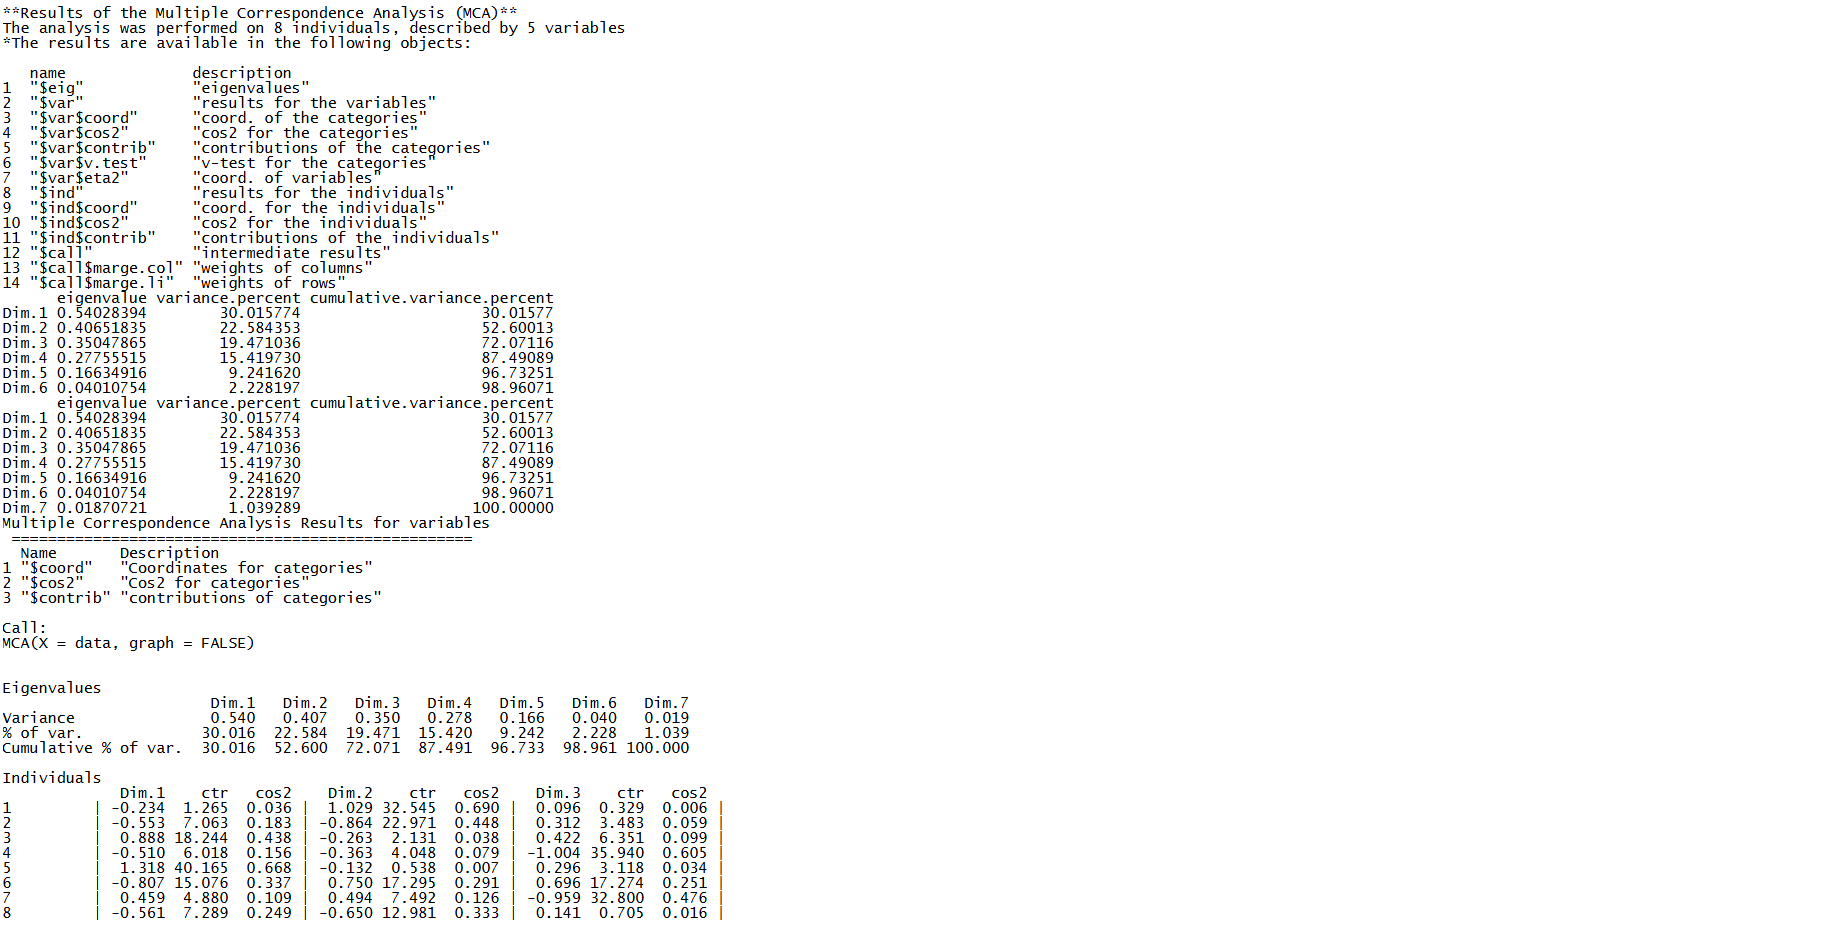
\includegraphics[width=0.95\textwidth]{ACM1.png}
    \caption{Résultats numériques de l'ACM - Partie 1 (valeurs propres, inertie)}
    \label{fig:acm1}
\end{figure}

\begin{figure}[H]
    \centering
    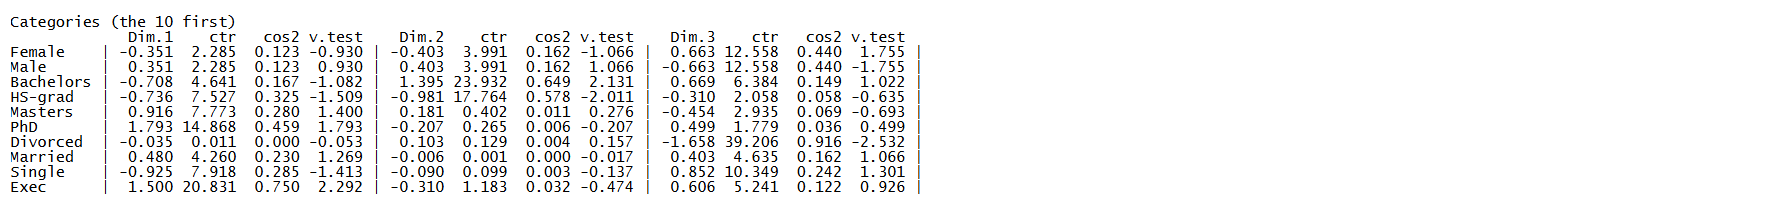
\includegraphics[width=0.95\textwidth]{ACM2.png}
    \caption{Résultats numériques de l'ACM - Partie 2 (coordonnées, contributions)}
    \label{fig:acm2}
\end{figure}

\begin{figure}[H]
    \centering
    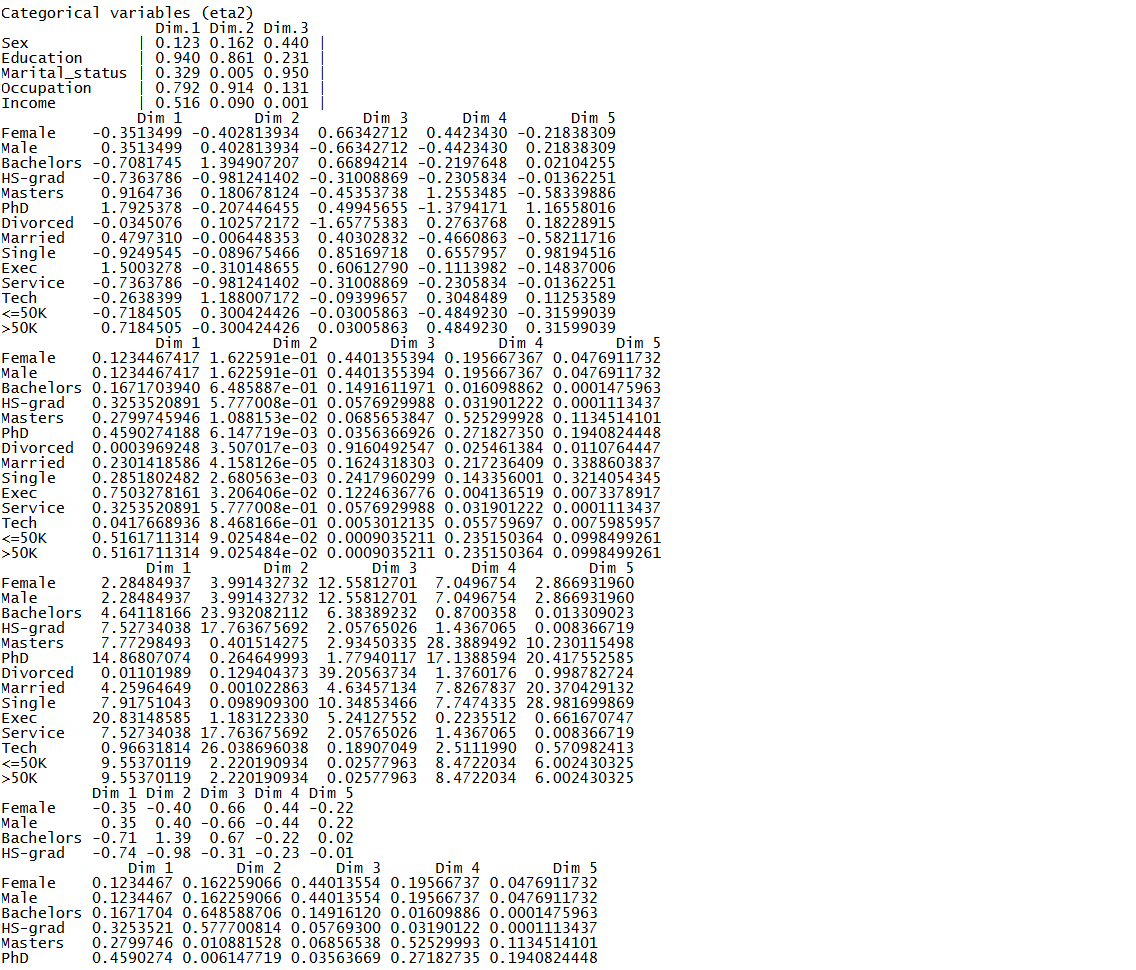
\includegraphics[width=0.95\textwidth]{ACM3.png}
    \caption{Résultats numériques de l'ACM - Partie 3 (cos², qualité de représentation)}
    \label{fig:acm3}
\end{figure}

\subsection{Graphiques de l'ACM}

\begin{figure}[H]
    \centering
    \includegraphics[width=0.9\textwidth]{"biplot acm.png"}
    \caption{Biplot de l'ACM : représentation simultanée des individus et des modalités}
    \label{fig:biplot}
\end{figure}

\begin{figure}[H]
    \centering
    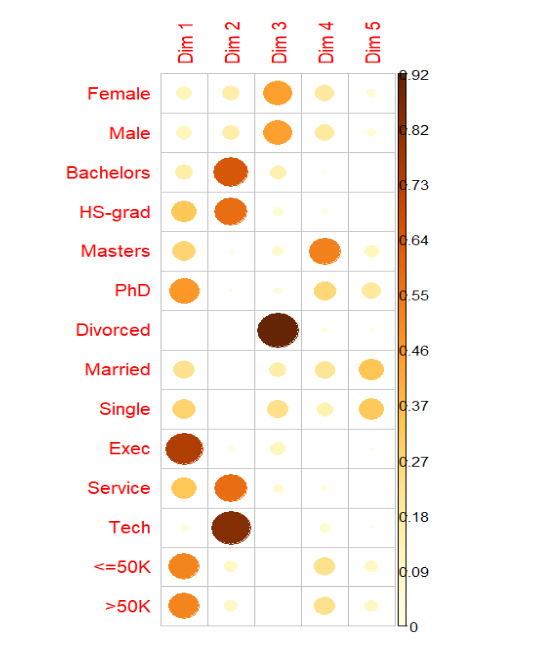
\includegraphics[width=0.9\textwidth]{indiv_varia.png}
    \caption{Graphique des individus et des variables catégorielles}
    \label{fig:indiv_var}
\end{figure}

\begin{figure}[H]
    \centering
    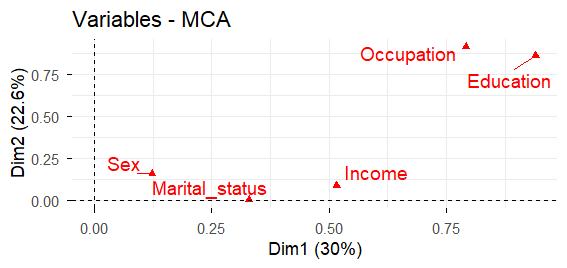
\includegraphics[width=0.9\textwidth]{variables_dimensions.png}
    \caption{Corrélation entre les variables et les dimensions principales}
    \label{fig:var_dim}
\end{figure}

\subsection{Coordonnées des modalités}

\begin{table}[H]
\centering
\caption{Coordonnées des modalités sur les 3 premiers axes}
\footnotesize
\begin{tabular}{|l|r|r|r|}
\hline
\textbf{Modalité} & \textbf{Dim.1} & \textbf{Dim.2} & \textbf{Dim.3} \\
\hline
Sex\_Female & -0.351 & -0.403 & -0.663 \\
Sex\_Male & 0.351 & 0.403 & 0.663 \\
Education\_Bachelors & -0.708 & 1.395 & -0.669 \\
Education\_HS-grad & -0.736 & -0.981 & 0.310 \\
Education\_Masters & 0.916 & 0.181 & 0.454 \\
Education\_PhD & 1.793 & -0.207 & -0.499 \\
Marital\_status\_Divorced & -0.035 & 0.103 & 1.658 \\
Marital\_status\_Married & 0.480 & -0.006 & -0.403 \\
Marital\_status\_Single & -0.925 & -0.090 & -0.852 \\
Occupation\_Exec & 1.500 & -0.310 & -0.606 \\
Occupation\_Service & -0.736 & -0.981 & 0.310 \\
Occupation\_Tech & -0.264 & 1.188 & 0.094 \\
Income\_$\leq$50K & -0.718 & 0.300 & 0.030 \\
Income\_$>$50K & 0.718 & -0.300 & -0.030 \\
\hline
\end{tabular}
\end{table}

\subsection{Contributions des modalités}

\begin{table}[H]
\centering
\caption{Contributions des modalités aux axes (\%)}
\footnotesize
\begin{tabular}{|l|r|r|r|}
\hline
\textbf{Modalité} & \textbf{Dim.1} & \textbf{Dim.2} & \textbf{Dim.3} \\
\hline
Sex\_Female & 2.28 & 3.99 & 12.56 \\
Sex\_Male & 2.28 & 3.99 & 12.56 \\
Education\_Bachelors & 4.64 & 23.93 & 6.38 \\
Education\_HS-grad & 7.53 & 17.76 & 2.06 \\
Education\_Masters & 7.77 & 0.40 & 2.93 \\
Education\_PhD & \textbf{14.87} & 0.26 & 1.78 \\
Marital\_status\_Divorced & 0.01 & 0.13 & \textbf{39.21} \\
Marital\_status\_Married & 4.26 & 0.00 & 4.63 \\
Marital\_status\_Single & 7.92 & 0.10 & 10.35 \\
Occupation\_Exec & \textbf{20.83} & 1.18 & 5.24 \\
Occupation\_Service & 7.53 & 17.76 & 2.06 \\
Occupation\_Tech & 0.97 & \textbf{26.04} & 0.19 \\
Income\_$\leq$50K & 9.55 & 2.22 & 0.03 \\
Income\_$>$50K & 9.55 & 2.22 & 0.03 \\
\hline
\end{tabular}
\end{table}

% ============================================
% INTERPRÉTATION
% ============================================
\section{Interprétation des Résultats}

\subsection{Interprétation des axes factoriels}

\subsubsection{Axe 1 : Niveau socio-professionnel (31.03\% d'inertie)}

Le premier axe factoriel oppose deux profils socio-économiques distincts :

\textbf{Côté positif (coordonnées $>$ 0) :}
\begin{itemize}
    \item \textbf{Occupation\_Exec} (1.500, contribution 20.83\%) : Les cadres exécutifs
    \item \textbf{Education\_PhD} (1.793, contribution 14.87\%) : Le plus haut niveau d'éducation
    \item \textbf{Education\_Masters} (0.916) : Diplômés de master
    \item \textbf{Income\_$>$50K} (0.718, contribution 9.55\%) : Revenus élevés
    \item \textbf{Marital\_status\_Married} (0.480) : Personnes mariées
\end{itemize}

\textbf{Côté négatif (coordonnées $<$ 0) :}
\begin{itemize}
    \item \textbf{Marital\_status\_Single} (-0.925) : Personnes célibataires
    \item \textbf{Education\_HS-grad} (-0.736) et \textbf{Occupation\_Service} (-0.736) : Niveau d'éducation secondaire et emplois de service
    \item \textbf{Income\_$\leq$50K} (-0.718) : Revenus modestes
    \item \textbf{Education\_Bachelors} (-0.708) : Licence
\end{itemize}

\textbf{Interprétation :} L'axe 1 représente un \textbf{gradient socio-professionnel}. Il oppose les individus à haut niveau d'éducation (PhD, Masters), occupant des postes de direction (Exec), avec des revenus élevés ($>$50K) et souvent mariés, aux individus de niveau d'éducation plus modeste (HS-grad), travaillant dans les services, avec des revenus plus faibles et souvent célibataires. C'est un axe de \textbf{stratification sociale}.

\subsubsection{Axe 2 : Type d'emploi technique vs service (23.35\% d'inertie)}

Le deuxième axe met en évidence une opposition entre types d'activités professionnelles :

\textbf{Côté positif :}
\begin{itemize}
    \item \textbf{Occupation\_Tech} (1.188, contribution 26.04\%) : Emplois techniques
    \item \textbf{Education\_Bachelors} (1.395, contribution 23.93\%) : Licence
    \item \textbf{Sex\_Male} (0.403) : Tendance masculine
    \item \textbf{Income\_$\leq$50K} (0.300) : Revenus modestes
\end{itemize}

\textbf{Côté négatif :}
\begin{itemize}
    \item \textbf{Education\_HS-grad} (-0.981) et \textbf{Occupation\_Service} (-0.981, contribution 17.76\%) : Niveau secondaire et services
    \item \textbf{Sex\_Female} (-0.403) : Tendance féminine
    \item \textbf{Income\_$>$50K} (-0.300) : Revenus élevés
\end{itemize}

\textbf{Interprétation :} L'axe 2 distingue les \textbf{profils techniques} (Tech + Bachelors, plutôt masculins) des \textbf{profils de service} (Service + HS-grad, plutôt féminins). Paradoxalement, les emplois de service semblent associés ici à des revenus plus élevés, ce qui peut s'expliquer par la petite taille de l'échantillon.

\subsubsection{Axe 3 : Situation familiale (20.13\% d'inertie)}

Le troisième axe est fortement marqué par le statut matrimonial :

\textbf{Côté positif :}
\begin{itemize}
    \item \textbf{Marital\_status\_Divorced} (1.658, contribution 39.21\%) : Personnes divorcées
    \item \textbf{Sex\_Male} (0.663, contribution 12.56\%) : Hommes
    \item \textbf{Education\_Masters} (0.454) : Master
\end{itemize}

\textbf{Côté négatif :}
\begin{itemize}
    \item \textbf{Marital\_status\_Single} (-0.852) : Célibataires
    \item \textbf{Sex\_Female} (-0.663, contribution 12.56\%) : Femmes
    \item \textbf{Education\_Bachelors} (-0.669) : Licence
\end{itemize}

\textbf{Interprétation :} L'axe 3 oppose principalement les \textbf{divorcés} (souvent masculins avec un niveau Master) aux \textbf{célibataires} (plutôt féminins avec un niveau Bachelors). Cet axe capture la dimension de la \textbf{trajectoire familiale}.

\subsection{Analyse des associations entre modalités}

\subsubsection{Profil 1 : Cadres supérieurs}

Les modalités suivantes sont proches sur le plan factoriel et définissent un profil cohérent :
\begin{itemize}
    \item \textbf{PhD / Masters} + \textbf{Exec} + \textbf{$>$50K} + \textbf{Married}
    \item Ce profil correspond aux \textbf{cadres supérieurs diplômés}, généralement mariés et avec des revenus confortables
\end{itemize}

\subsubsection{Profil 2 : Employés de service}

Un autre groupe de modalités forme un profil distinct :
\begin{itemize}
    \item \textbf{HS-grad} + \textbf{Service} + \textbf{Female}
    \item Ce profil représente les \textbf{employées du secteur des services} avec un niveau d'éducation secondaire
\end{itemize}

\subsubsection{Profil 3 : Techniciens}

\begin{itemize}
    \item \textbf{Bachelors} + \textbf{Tech} + \textbf{Male} + \textbf{Single}
    \item Ce profil correspond aux \textbf{techniciens diplômés}, souvent masculins et célibataires
\end{itemize}

\subsection{Qualité de représentation (Cos²)}

Les modalités les mieux représentées sur le plan (Dim.1, Dim.2) sont :
\begin{itemize}
    \item \textbf{Occupation\_Tech} : Cos² = 0.847 sur Dim.2 (excellente représentation)
    \item \textbf{Occupation\_Exec} : Cos² = 0.750 sur Dim.1 (très bonne représentation)
    \item \textbf{Education\_Bachelors} : Cos² = 0.649 sur Dim.2 (bonne représentation)
    \item \textbf{Education\_HS-grad} : Cos² = 0.578 sur Dim.2 (bonne représentation)
    \item \textbf{Income} : Cos² = 0.516 sur Dim.1 (représentation correcte)
\end{itemize}

Les modalités avec un faible Cos² (comme Sex sur les deux premiers axes) nécessitent l'examen des axes suivants pour être correctement interprétées.

\subsection{Synthèse de l'interprétation}

L'ACM appliquée aux données Adult Clean révèle plusieurs structures importantes :

\begin{enumerate}
    \item \textbf{Stratification socio-professionnelle} (Axe 1) : Une opposition claire entre les profils à haut capital éducatif et professionnel (PhD, Exec, $>$50K) et les profils plus modestes (HS-grad, Service, $\leq$50K).
    
    \item \textbf{Segmentation par type d'activité} (Axe 2) : Une distinction entre les métiers techniques (Tech, Bachelors, masculin) et les emplois de service (Service, HS-grad, féminin).
    
    \item \textbf{Dimension familiale} (Axe 3) : L'impact du statut matrimonial, avec une opposition divorcés/célibataires liée au genre.
    
    \item \textbf{Cohérence des profils} : Les associations observées sont sociologiquement pertinentes (éducation-profession-revenu forment un ensemble cohérent).
    
    \item \textbf{Limites} : La petite taille de l'échantillon (8 individus) invite à la prudence dans la généralisation des résultats.
\end{enumerate}

% ============================================
% CODES
% ============================================
\section{Codes R et Python}

\subsection{Code R}

\begin{lstlisting}[style=Rstyle, caption={Code R pour l'ACM avec FactoMineR et factoextra}]
# Chargement des librairies necessaires
library(readxl)
library(FactoMineR)
library(factoextra)
library(corrplot)

# Chargement des donnees
adult_clean <- read_excel("adult_clean.xlsx")
data <- adult_clean
attach(data)

# Realisation de l'ACM sur les variables actives
res.mca <- MCA(data, graph = FALSE)
print(res.mca)

# Extraction des valeurs propres
eig.val <- get_eigenvalue(res.mca)
print(eig.val)

# Graphique de l'inertie (eboulis des valeurs propres)
fviz_screeplot(res.mca, addlabels = TRUE, ylim = c(0, 45))

# Biplot des individus et des modalites
fviz_mca_biplot(res.mca, repel = TRUE, 
                ggtheme = theme_minimal())

# Extraction des resultats sur les variables
var <- get_mca_var(res.mca)

# Coordonnees des modalites
print(var$coord)

# Qualite de representation (Cos2)
print(var$cos2)

# Contributions des modalites aux axes
print(var$contrib)

# Graphique des correlations variables-dimensions
fviz_mca_var(res.mca, choice = "mca.cor", 
             repel = TRUE, 
             ggtheme = theme_minimal())

# Graphique des modalites colorees par Cos2
fviz_mca_var(res.mca, col.var = "cos2",
             gradient.cols = c("#00AFBB", "#E7B800", "#FC4E07"), 
             repel = TRUE,
             ggtheme = theme_minimal())

# Visualisation du Cos2 avec corrplot
corrplot(var$cos2, is.corr = FALSE)
\end{lstlisting}

\subsection{Code Python}

\begin{lstlisting}[style=Pythonstyle, caption={Code Python pour l'ACM avec prince}]
# Chargement des librairies
import pandas as pd
import numpy as np
import matplotlib.pyplot as plt
import prince

# Chargement des donnees
data = pd.read_excel("adult_clean.xlsx")

# Affichage des informations sur les donnees
print("Dimensions :", data.shape)
print("\nVariables :", data.columns.tolist())
print("\nApercu des donnees :")
print(data.head())

# Realisation de l'ACM avec prince
mca = prince.MCA(
    n_components=5,      # Nombre de dimensions
    n_iter=3,            # Iterations pour convergence
    random_state=42      # Reproductibilite
)
mca = mca.fit(data)

# Valeurs propres et inertie
eigenvalues = mca.eigenvalues_
total_inertia = sum(eigenvalues)
variance_pct = eigenvalues / total_inertia * 100
cumulative = np.cumsum(variance_pct)

print("\n=== VALEURS PROPRES ===")
for i, (eig, var, cum) in enumerate(zip(eigenvalues, 
                                         variance_pct, 
                                         cumulative)):
    print(f"Dim.{i+1}: {eig:.3f} ({var:.2f}%, cumul: {cum:.2f}%)")

# Coordonnees des modalites
print("\n=== COORDONNEES DES MODALITES ===")
col_coords = mca.column_coordinates(data)
print(col_coords.round(3))

# Contributions des modalites (en pourcentage)
print("\n=== CONTRIBUTIONS (%) ===")
col_contrib = mca.column_contributions_ * 100
print(col_contrib.round(2))

# Qualite de representation (Cos2)
print("\n=== COS2 ===")
col_cos2 = mca.column_cosine_similarities(data)
print(col_cos2.round(3))

# Coordonnees des individus
print("\n=== COORDONNEES DES INDIVIDUS ===")
row_coords = mca.row_coordinates(data)
print(row_coords.round(3))

# Visualisation du biplot
ax = mca.plot(
    data,
    x_component=0,
    y_component=1,
    show_column_markers=True,
    show_row_markers=True,
    show_column_labels=True
)
plt.title("Biplot ACM - Dimensions 1 et 2")
plt.tight_layout()
plt.savefig("acm_biplot_python.png", dpi=150)
plt.show()
\end{lstlisting}

% ============================================
% CONCLUSION
% ============================================
\section{Conclusion}

L'Analyse des Correspondances Multiples appliquée aux données Adult Clean a permis de :

\begin{enumerate}
    \item \textbf{Identifier trois dimensions structurantes} : le niveau socio-professionnel (Axe 1), le type d'activité professionnelle (Axe 2), et la situation familiale (Axe 3), expliquant ensemble 74.5\% de l'inertie totale.
    
    \item \textbf{Mettre en évidence des profils types} : cadres supérieurs diplômés et mariés, employées de service de niveau secondaire, techniciens diplômés célibataires.
    
    \item \textbf{Révéler des associations cohérentes} : la forte liaison entre niveau d'éducation, type d'occupation et niveau de revenu confirme les théories de stratification sociale.
    
    \item \textbf{Souligner l'importance du genre} : les femmes sont davantage représentées dans les services tandis que les hommes dominent les emplois techniques.
\end{enumerate}

\textbf{Limites :} La taille réduite de l'échantillon (8 observations) limite la portée des conclusions. Une analyse sur un échantillon plus conséquent permettrait de confirmer ces tendances.

\end{document}
